\chapter{Simulating dynamics of quantum system using D-Wave annealer}
\label{chapter:simulating}

The leading motivation behind the development of quantum computing devices is simulating quantum systems intractable by classical computers. But how far are we from this goal? This chapter presents a possible approach for simulating quantum systems (or any time-dependent dynamical system) that can be used with annealing devices such as D-Wave quantum annealer or Fujitsu digital annealer. To illustrate the working of our algorithm, we simulate the simplest single-qubit system and demonstrate that already near-term annealing devices are capable of capturing its dynamics in some regime of parameters.

\section{Parallel in time simulation of quantum systems}
Problems solved by annealers exhibit no time dependence. Therefore, simulating any time-dependent phenomena using those devices requires reformulating the problem as one that is static in nature. In our case, it is possible by enlarging the Hilbert space of the system under consideration, so that the states of this larger space encode also temporal information.

Let us first start by precisely defining the problem we want to address.
Consider a $L$ dimensional real or complex dynamical system whose behavior is determined by the following partial differential equation
\begin{equation}
\label{eq:dynamical-system}
    \frac{\partial \ket{\psi(t)}}{\partial t} = K(t) \ket{\psi(t)}
\end{equation}

Here, $\ket{\psi(t)}$ denotes the system's state at time $t$ and operator $K$ is the so--called Hamiltonian. It is clearly visible that an isolated quantum systems can be described by equation \eqref{eq:dynamical-system}, as putting $K=-\frac{i}{\hbar}H$ transforms it into Schr\"{o}dinger equation.

Given an initial state $\ket{\psi(t_0)}$ the equation \eqref{eq:dynamical-system}
admits a unique solution. Namely,
\begin{equation}
    \ket{\psi(t)} \coloneqq U(t, t_0) \ket{\psi(t_0)},
\end{equation}
where operator $U(t, t_0)$ is a propagator transforming the initial state of
the system into its state at time $t$ and is given by
\begin{equation}
    \label{eq:propagator}
    U(t, t_0) = \altmathcal{T} \exp \left( \int_{t_0}^t K(\tau)d\tau \right).
\end{equation}
Here, $\altmathcal{T}$ denotes the well-known time-ordering operation.
Note that in the case when $K(t)$ commutes with $K(t')$ for every $t' \ne t$, the
time-ordering can be omitted. In particular, this is the case if $K$ is time
independent.

Given the initial state we are interested in finding the state of the
system at some time $t > t_0$. Numerical methods for solving this problem
usually start by partitioning the interval $[t_0, t]$ into $N$ distinct time
points $t_0 < t_1 < \ldots < t_{N-1}$. Then, the desired state $\ket{\psi(t)}$
can be computed as
\begin{equation}
\ket{\psi(t)} = U(t_{N-1}, t_{N-2}) \cdots U_{n+1}U_n \cdots U_0 \ket{\psi(t_0)}.
\end{equation}
This is purely a rearrangement of computations which by itself gives no benefit
over applying $U(t, t_0)$ directly. However, shortening the interval allows for a more efficient approximation of propagators, which can be done using a variety of methods (e.g. via Suzuki-Trotter approximation).

This procedure, common to many sequential methods, gives a starting point for a class of the so--called parallel in--time methods based on the Feynmann clock operator. In this approaches one starts by suitably enlarging state space so that it can encode the state of the system at all times $t_0, t_1, \ldots, t_{N-1}$. This can be done by considering a tensor product of a state space with the new Hilbert space spanned by the orthonormal basis $\{\ket{0}, \ket{1}, \ldots, \ket{N-1}\}$. Then, the following superposition encodes states of the system in all $N$ moments of time
\begin{equation}
    \ket{\Psi} = \sum_{n=0}^{N-1} \ket{n} \otimes \ket{\psi(t_n)}.
\end{equation}
The solution to the original problem can be then obtained using so--called \emph{clock operator}
\begin{equation}
\label{eq:clock2}
 \clockop
   =
\sum_{n=0}^{N-2}
\big(
\ket{t_{n+1}}\bra{t_{n+1}} \otimes I - \ket{t_{n+1}}\bra{t_n} \otimes U_n
+ \text{h.c.}
\big).
\end{equation}
Indeed, one can see that $\ket{\Psi}$ becomes a solution to eigenequation
\begin{equation}
\label{eq:clock-eigenequation}
\clockop \ket{\Psi} = 0.
\end{equation}
Note, however, that equation \eqref{eq:clock-eigenequation} does not take into account in any way an initial state of the system at $t_0$. Therefore, $\ket{\Psi}$ is not its unique eigenvector. It is possible to fix this problem by adding a \emph{penalty} term $\clockop_0 = \ket{t_0}\bra{t_0}\otimes(I-\ket{\psi_0}\bra{\psi_0})$ to the left hand side. The equation to solve becomes then $(\clockop + \clockop_0) \ket{\Psi} = 0$.
This equation can be reformulated as
\begin{equation}
\label{eq:gsys}
\coefmatrix \ket{\Psi}
=
\ket{t_0}\otimes \ket{\psi_0} = \ket{\Phi},
\quad
\coefmatrix=\clockop + \ket{t_0}\bra{t_0} \otimes I.
\end{equation}
Thus, using an approximation of evolution operators, we constructed a system of linear equations encoding the solution to the equation \eqref{eq:dynamical-system} under the given initial condition. At this point, however, it is not possible to solve it using a quantum annealer yet. To do so, one first needs to convert this system into an optimization problem
with binary variables, which is what we will deal with next.
\section{Solving systems of linear equations as an optimization problem}
There is a straightforward way of converting equation \eqref{eq:gsys} into
an optimization problem. One can observe that if the solution minimizes the norm $\left\Vert \coefmatrix\ket{\mathbf{x}} - \ket{\Phi}\right\Vert$.
Since the norm is non-negative, it follows that solving equation \eqref{eq:gsys} is equivalent to the following optimization problem
\begin{equation}
    \label{eq:optimize_1}
    \ket{\Psi} = \argmin_{\mathbf{x}} f(\mathbf{x}), \quad f({\mathbf x}) = \left\Vert \coefmatrix\ket{\mathbf{x}} - \ket{\Phi}\right\Vert^2.
\end{equation}
However, $f$ in the equation \eqref{eq:optimize_1} is not the only choice of a target function. If $\coefmatrix$ is positive-definite, one can consider the following function $h$ instead
\begin{equation}
\label{eq:optimize_2}
h(\mathbf{x})=\frac{1}{2}\bra{\mathbf{x}}\coefmatrix\ket{\mathbf{x}} -
\braket{\mathbf{x}}{\Phi}.
\end{equation}
It is easy to verify that solution to \eqref{eq:gsys} also minimizes $h$ by computing its gradient and Hessian
\begin{equation}
    \nabla h(\mathbf{x}) = \coefmatrix\ket{\mathbf{x}}-\ket{\Phi}, \quad \nabla^2 h({\mathbf
x})=\coefmatrix>0
\end{equation}
Since hessian is positive and $\ket{\Psi}$ is the only vector at which $\nabla h$ vanishes, it follows that $\ket{\Psi}$ is indeed a global minimum of $h$.

\section{Discretizing variables}
So far we have been working with continuous variables. The next necessary step before solving optimization problems \eqref{eq:optimize_1} and \eqref{eq:optimize_2} using annealer is converting them in such a way that all unknowns are dichotomous. The idea is to express each of the unknown coefficients of $\ket{\mathbf{x}} = $[$x_1, \ldots, x_{LN}]^T$ in  fixed-point approximation. If one  assumes (binary) order of magnitude of coefficients of $\mathbf x$ to be $D$ (i.e. $x_i \in [-2^D, 2^D]$ for each $i$), then it can be approximated up to $R$ bits of precision as
\begin{equation}
\label{eq:fixed}
    x_i \approx 2^D \left(2 \sum_{\alpha=0}^{R-1}2^{-\alpha}q_i^{\alpha} -1\right).
\end{equation}
Here variables $q_i^\alpha$ are consecutive bits of the fixed-points expansion of $x_i$. Note that approximation of $x_i$ in \eqref{eq:fixed} is a linear combination of its bits, therefore plugging it into optimization problems \eqref{eq:optimize_1} and \eqref{eq:optimize_2} yields
quadratic unconstrained optimization problems of the form
\begin{align}
\label{eq:qubo_f}
\argmin_{\mathbf{q}} f(\mathbf{q}) = \argmin_{\mathbf{q}} \sum_{i,\alpha} c_i^{\alpha} q_i^r + \sum_{i,j,\alpha,\beta} d_{ij}^{\alpha\beta} q_i^{\alpha} q_j^{\beta} + f_0,\\
\label{eq:qubo_h}
\argmin_{\mathbf{q}} h(\mathbf{q}) = \argmin_{\mathbf{q}} \sum_{i,\alpha} a_i^{\alpha} q_i^r + \sum_{i,j,\alpha,\beta} b_{ij}^{\alpha\beta} q_i^{\alpha} q_j^{\beta} + h_0.
\end{align}
Coefficients in equations \eqref{eq:qubo_f} and \eqref{eq:qubo_h} can be straightforwardly computed by an appropriate substitutions into equations \eqref{eq:optimize_1} and \eqref{eq:optimize_2}. For brevity, here we present only the formulas for the equation \eqref{eq:qubo_h}, which reads
\begin{eqnarray}
\begin{split}
b_{ij}^{\alpha\beta} &= \coefmatrix_{ij} 2^{1-\alpha-\beta+2D} \\
a_i^\alpha &= \left( 2^{-\alpha+D}\coefmatrix_{ii} - 2^D\sum_{j}\coefmatrix_{ij}- \Phi_i\right)2^{1-\alpha+D},
\\
h_0 &= 2^D\left( 2^{D-1}\sum_{ij}\coefmatrix_{ij}+\sum_i \Phi_i\right).
\end{split}
\label{eq:coeff}
\end{eqnarray}

Our approach requires the order of magnitude $D$ and precision $R$ in equation \eqref{eq:fixed} to be chosen beforehand. Choosing the right $D$ requires knowledge of the range in which coefficients lie. If its value is too small, the approximations will fail to capture the most significant bits of the real solution.
On the other hand, choosing $D$ that is too large will result in wasting variables for encoding insignificant zeros. Fortunately, for many systems a suitable $D$ can be determined. For instance, for qubit and multi-qubit systems, each $x_i$ is bounded by $\pm 1$ which makes $D=0$ the optimal choice for this case.

QUBOs in the equations \eqref{eq:qubo_f} and \eqref{eq:qubo_h} are defined on the graph of size $N \cdot R \cdot L$. The number of edges (i.e. nonzero quadratic terms) depends on the number of nonzero off-diagonal elements of matrix $\coefmatrix$. It is interesting to note that the overall density of the graph is an increasing function of $R$ (bigger precision requires a denser graph) while on the other hand, it is a decreasing function of $L$ (larger systems require sparser graphs).

We converted the original problem of finding the dynamics of the system into a binary optimization problem suitable for input to the quantum annealer. In the next section, we will discuss experiments that we performed using D-Wave 2000Q\_2\_1 and D-Wave 2000Q\_5 machines to test the above-described approach.


\section{Parallel-in-time simulations with quantum annealer}
Before discussing the results of our experiments, let us focus first on its design. To exemplify our approach we chose to simulate the dynamics of a two--level system with an initial state $\ket{0}$ and a hamiltonian
$$
H = \frac{\pi}{2}\sigma_y,
$$
where $\sigma_y$ is a Pauli spin operator in the $y$-direction.
This particular choice of Hamiltonian and initial state makes the system suitable for implementation on present-day quantum annealers for several reasons. One can easily see that the evolution of the system is real (as opposed to complex), which halves the number of needed variables. Secondly, for integral time points $t_0=0, t_1=1, \ldots$ coefficients of the wave function can be expressed \emph{exactly} using only two bits of precision per coefficient, which further reduces the number of needed variables.

\begin{figure}[!h]
    \centering
    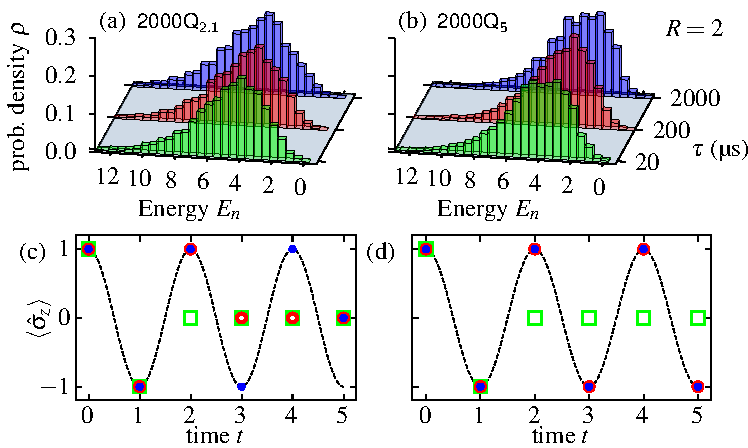
\includegraphics{figures/fig2.pdf}
    \caption{(a)--(b) Energy distribution of samples obtained from D-Wave annealers for different annealing times $\tau$. Notice a slight shift of distributions towards the ground state for the 2000Q\_{5} device. (c)--(d) Rabi oscillations of the simulated system. The obtained samples were normed before plotting. As can be seen in panel (d), the low-noise device was able to faithfully capture oscillations for $\tau=200, 2000$.
    The annealing time ($\tau=$
    \tikzquad\,\,\, -- 20,
    \,\tikzcircle\,\,\,-- 200,
    \,\tikzdot\,\,-- 2000)
      is measured in microseconds.
    }
    \label{fig:energy-hist}
\end{figure}
\todo{Add units to annealing time}
We simulated the above system using values of $R=2, 3$ and for several numbers of time points $N$. We used annealing time $\tau$ spanning several orders of magnitude, namely $\tau=20\mu s, 200 \mu s, 2000 \mu s$. Since the resulting graphs were dense, we decided to use standard embedding of the complete graph $K_n$ on Chimera. To assess the quality of solutions obtained from the annealer, we sampled each problem $10^4$ times on  DW-2000Q\_{2.1} devices as well as its low-noise version DW-2000Q\_{5}. Energy distributions of samples obtained for $N=6$ are depicted in Fig. \ref{fig:energy-hist}. The same figure also illustrates the dynamics of the expected value of $\sigma_z$ for the lowest energy sample obtained for a given annealing time. Note that to present a physical meaning of the decoded solution, it was normed before plotting.

For comparison with the low-noise annealer, we also solved the resulting optimization problems using CPLEX and a recent Tensor Networks--based sampler. The results of this comparison are depicted in Fig. \ref{fig:cplex_tn_dwave}.

Results depicted in figures \ref{fig:energy-hist} and \ref{fig:cplex_tn_dwave} show, that the DW-2000Q\_{5} was able to faithfully capture dynamics of qubit if the state of the system was encoded using $R=2$ bits of precision per coefficient when the annealing time $\tau=200$ was used. For larger values of $N$ and $R$ one can observe noticeable degradation in the quality of the solution.

\begin{figure}
    \centering
    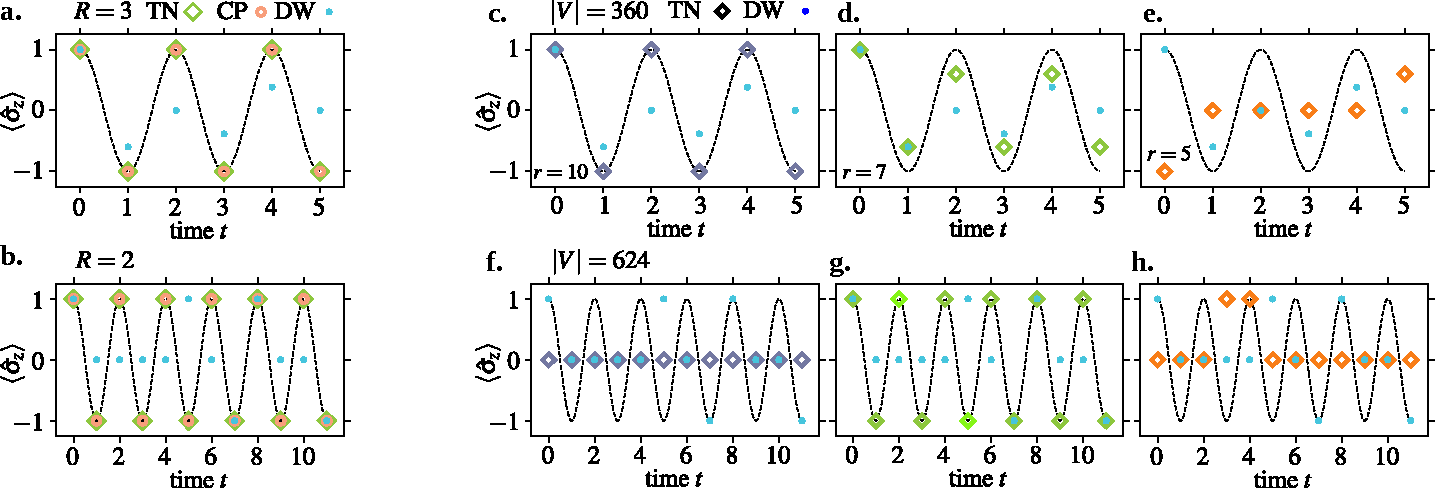
\includegraphics[width=\textwidth]{figures/fig34_merge.pdf}
    \caption{Caption}
    \label{fig:cplex_tn_dwave}
\end{figure}


%%% Local Variables:
%%% mode: latex
%%% TeX-master: "../main"
%%% End:
